\documentclass[11pt, a4paper]{article}

\usepackage[margin=1in]{geometry}
\usepackage{mathtools}
\usepackage{amsmath}
\usepackage{amssymb}
\usepackage{amsthm}
\newtheorem{newdef}{Definition}
\newtheorem{lemma}{Lemma}
\usepackage{graphicx}
\graphicspath{{./plots/}}
\usepackage{caption}
\usepackage{mwe}
\usepackage{subfig}
\usepackage{url}
\usepackage{float}
\usepackage{parskip}
\usepackage{fancyhdr}
\pagestyle{fancy}
\fancyhead{}
\lhead{CHAN Cissy Hiu Ying}
\rhead{Statistical Pattern Recognition (M3S7) Project}


\title{Statistical Pattern Recognition (M3S7) Project}
\author{CHAN Cissy Hiu Ying \\ Imperial College London}
\date{Autumn 2013/2014}


\newcommand{\E}{\mathrm{E}}
\newcommand{\Var}{\mathrm{Var}}
\newcommand{\Cov}{\mathrm{Cov}}
\newcommand{\bias}{\mathrm{bias}}
\newcommand{\bSigma}{\boldsymbol{\Sigma}}
\newcommand{\bmu}{\boldsymbol{\mu}}
\renewcommand{\qedsymbol}{$\blacksquare$}

\begin{document}

\vspace*{4cm}
{\let\newpage\relax\maketitle}
\newpage

\newpage
\tableofcontents

\newpage

\begin{abstract}
This project explores four statistical pattern recognition classifiers -- linear discriminant analysis, quadratic discriminant analysis, k nearest neighbours, and multi-layer perceptron. Using a sample data set of 2 classes and 28 features, each classifier is tested for its accuracy, complexity, and interpretability.

\end{abstract}

\newpage

\section{The data}
\subsection{A quick glance}

We are given the data set which can be found at
\begin{verbatim}
www2.imperial.ac.uk/~eakc07/S7/data6.dat
\end{verbatim}

A quick command tells us the dimensions of the data set:

\begin{quote}
\begin{verbatim}
> dim(data6)
[1] 1102   29
\end{verbatim}
\end{quote}

with the first column being the class labels consisting of 0 and 1. So we are dealing with a 2-class problem, with a set of 1102 observations of 28 dimensions.

We then split the data randomly into a training set and a test set of 1002 and 100 observations respectively. From this point on until Section 3, wherever "data" or equivalent is mentioned, it refers to the training set. To get a better picture of what we're dealing with, we plot each individual feature vector. As our data is organised by the classes, roughly the first half of the points belong to one class and the second half the other.

\begin{figure}[H]
\centering
	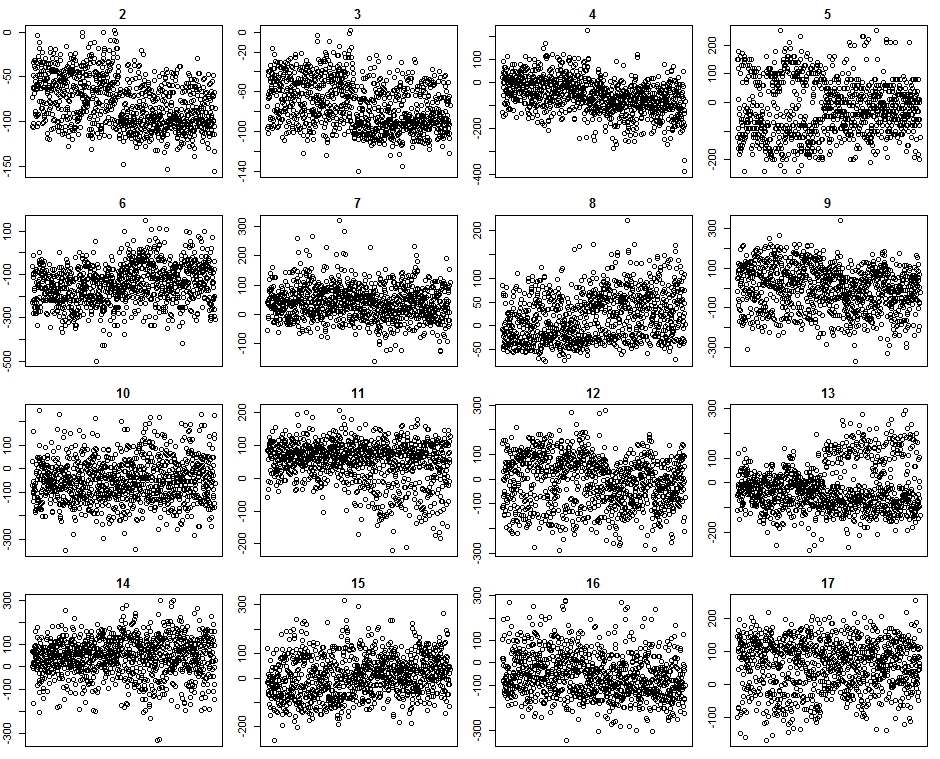
\includegraphics[scale=0.4]{featurevectors1.jpeg}
	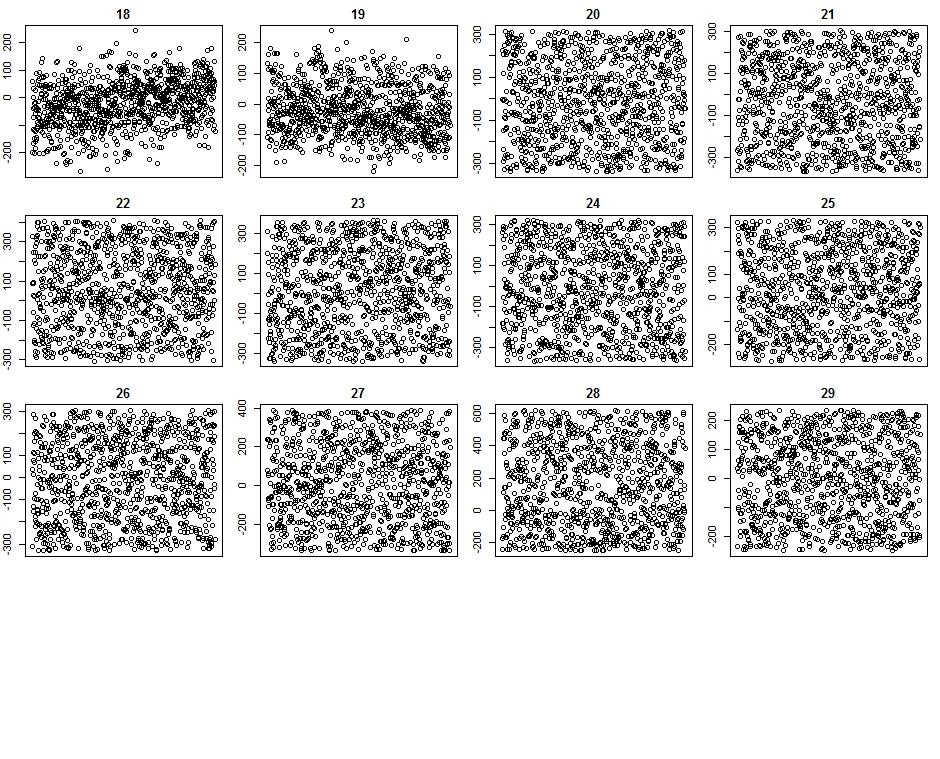
\includegraphics[scale=0.4,trim={0 6cm 0 0},clip]{featurevectors2.jpeg}
\caption{Individual feature vectors; titles show the feature vector number, x-axis is the observations}
\end{figure}

At a glance, features 2-9, 11-13 show a somewhat noticeable division by class, whereas the rest have no obvious class patterns (in fact features 20-29 appear to be distributed randomly and identically) but there may be connections between features that may be not apparent at this stage.

\subsection{Missing data}
There are some missing entries in our data, and a quick summary given below of the number of missing points in each feature tells us that there is at least one missing point in every feature, and also that there aren't actually that many.

\begin{quote}
\begin{verbatim}
 V2  V3  V4  V5  V6  V7  V8  V9 V10 V11 V12 V13 V14 V15 
  8   3   5   2   4   2   1   1   3   2   2   5   3   2
  
 V16 V17 V18 V19 V20 V21 V22 V23 V24 V25 V26 V27 V28 V29
   2   2   5   3   2   2   3   2   1   4   4   2   6   5 
\end{verbatim}
\end{quote}

Also, altogether, 85 observations out of 1002 contain at least one missing entry, with 41 from class 0 and 44 from class 1, which means that missing data aren't biased towards one class. There are ways to deal with  missing data, such as looking at the mean and variance of each feature, or make an educated guess for the missing entry taking into account the entries in other features for the same observation. However, since we have no real information on the features themselves, we cannot make an informed judgment to substitute the missing data, and also considering the number of missing entries and their distribution amongst data, we can afford to remove the observations, so we will.

\section{Using the training set}

Now we move on to proper classification methods on our training set.

\subsection{Parametric density estimation: linear discriminant analysis}
We will start by using one the most straight-forward classifier: the linear discriminant analysis (LDA), which is based on the Fisher criterion. This method is typically called a \emph{machine learner}, as it assumes that the class-conditional densities are multi-variate normal, estimates the parameters, and computes the log-likelihood of new data and assigns them to classes depending on the threshold. We will perform feature selection to the data prior to running the classifiers.

\subsubsection{Tuning features: best individual features}
Best individual features is a simple method but can be effective in terms of weeding out the features that may not be as useful. Its drawback is that it assumes that the features are uncorrelated, and hence for highly-correlated data it may actually give worse results. However, we shall see later that the selected features do indeed produce better error rates than using the entire data set.

For the purpose of feature selection, we will split the data into a training set of 992 observations and a test set of 100 observations, and use the cross-validation error rate to compare the performances. 

Next, we assign a score to each individual feature, calculated by 1 minus its individual cross-validation error rate using LDA, and arrange them in order of magnitude. The plot below shows the scores for each feature, which is what we would expect after examining each feature.

\begin{figure}[H]
\centering
	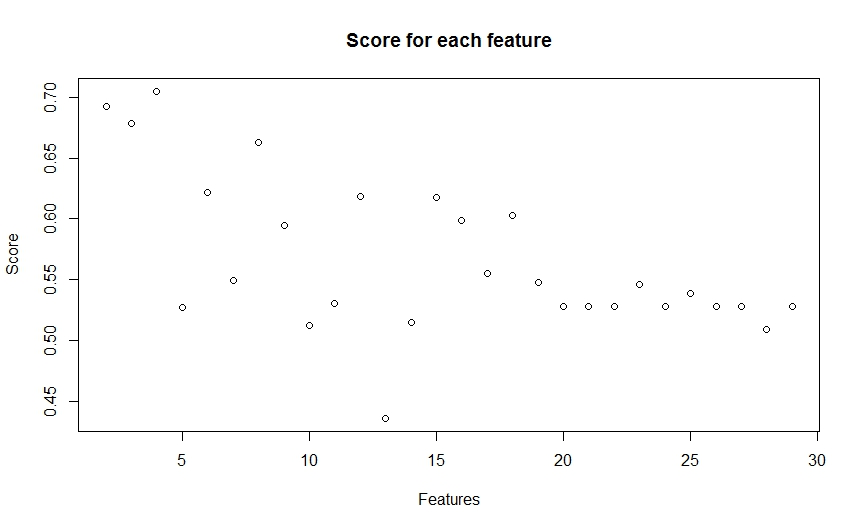
\includegraphics[scale=0.4]{ldacv1.jpeg}
\caption{Scores for each feature}
\end{figure}

In this case, lower is better. Then we then run the features through cross-validation again to find out the best number of features to use that minimises the error. We get the following plot:

\begin{figure}[H]
\centering
	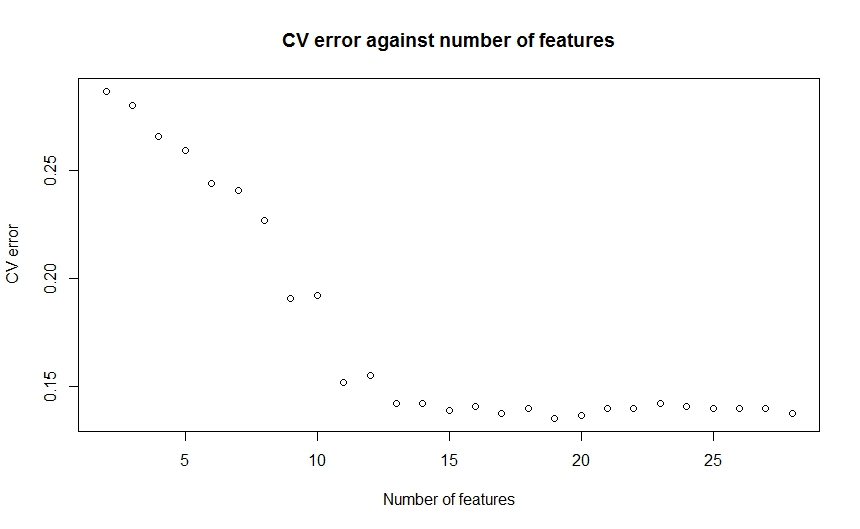
\includegraphics[scale=0.4]{ldacv2.jpeg}
\caption{CV errors; best individual features}
\end{figure}

We see that 19 features will gives us the minimum error of 13.5\%, and the features are the following:

\begin{quote}
\begin{verbatim}
> c
 [1]  4  2  3  8  6 12 15 18 16  9 17  7 19 23 25 11 20 21 22
\end{verbatim}
\end{quote}

Using the leave-one-out cross-validation error rate using all features is 13.7\%, whereas that for selected features is 13.5\%, a slight improvement.

\subsubsection{Assessment}

\underline{Apparent error}
\\
The apparent error using the selected features is 0.12759.

\underline{Hold-out error}
\\
The hold-out error rate is 0.13.

\underline{Leave-one-out cross validation error}
\\
The cross-validation error rate is 0.1352236.

\underline{10-fold cross validation error}
\\
We split the data into 10 equal sets and perform 10-fold cross-validation to get the average out-of-sample error rate of 0.143956.


\subsection{Parametric density estimation: quadratic discriminant analysis}

Next, we will try a method similar to LDA, the quadratic discriminant analysis (QDA).

We will see later that QDA performs significantly better than LDA. It tends to fit data better than LDA, as it has less constraints for covariance matrices, but a drawback is that it requires more parameters and may lead to weaker predictability power when the number of data is small, although in this case we are in no short of data. 

We will apply the same feature selection used for LDA here.

\subsubsection{Tuning parameters: best individual features}

We will run the best individual features algorithm through all the features again, this time the score calculated by the 1 minus cross-validation error using QDA.

\begin{figure}[H]
\centering
	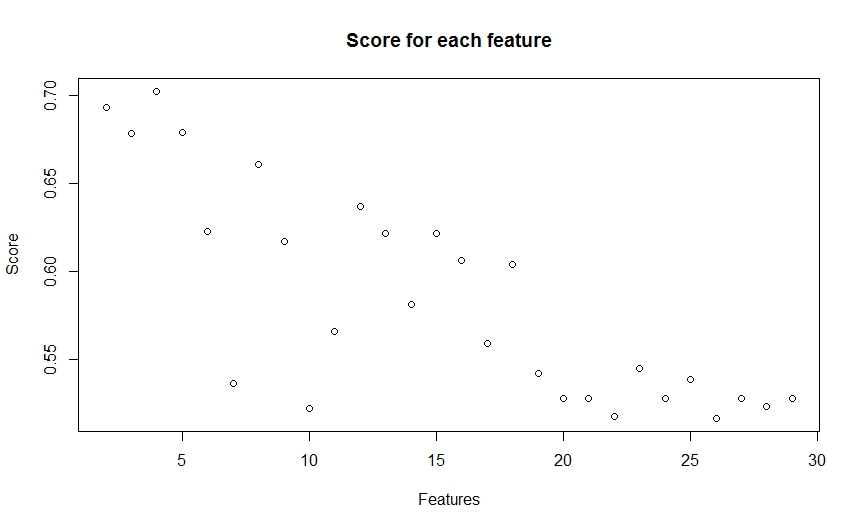
\includegraphics[scale=0.4]{qdacv1.jpeg}
\caption{Scores for each feature}
\end{figure}

\begin{figure}[H]
\centering
	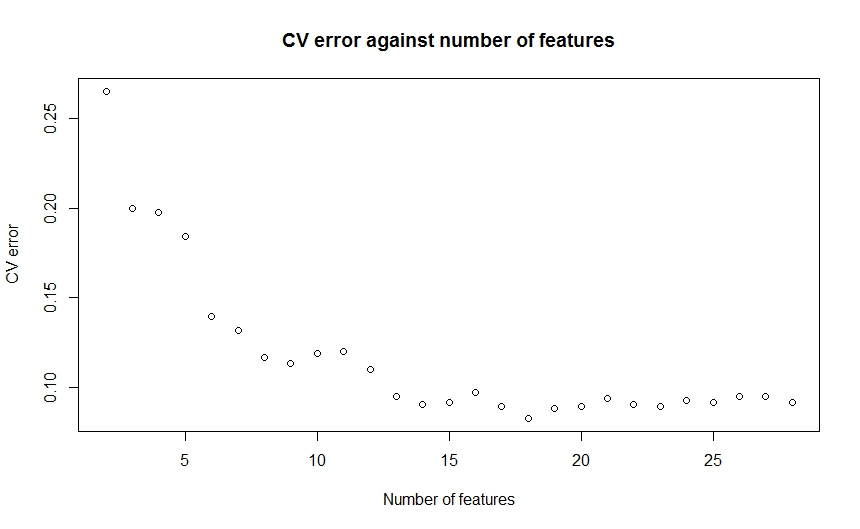
\includegraphics[scale=0.4]{qdacv2.jpeg}
\caption{CV errors; best individual features}
\end{figure}

In this case, the best number of features to use is 18, and the features are the following:

\begin{quote}
\begin{verbatim}
> c
 [1]  4  2  5  3  8 12  6 13 15  9 16 18 14 11 17 23 19 25
\end{verbatim}
\end{quote}

Again, the leave-one-out cross-validation error given when using all features is 9.16\%, whereas the same error rate given when using the selected features is 8.29\%.

\subsubsection{Assessment}

\underline{Apparent error}
\\
The apparent error using the selected features is 0.06324973.

\underline{Hold-out error}
\\
The hold-out error rate is 0.09.

\underline{Leave-one-out cross validation error}
\\
The cross-validation error rate is 0.08287895.

\underline{10-fold cross validation error}
The 10-fold cross-validation error rate is 0.0.08461538.


\subsection{Non-parametric density estimation method: k nearest neighbours}
We will try a non-parametric density estimation method, the $k$ nearest neighbours (KNN) method using the Euclidean distance. Unlike the other classifiers, KNN is sometimes dubbed \emph{lazy learner}, in that in doesn't perform any analysis on the data (no "learning") until it needs to classify new data.

The merits of KNN is that it is consistent, and it can be proven that as the number of observations tends towards infinity, the KNN error rate is less than or equal to twice the Bayes error rate.

However, a drawback of KNN is that it is localised and disregards the "big picture" in which all the data points are concerned, and that it must retain large amounts of data to classify a data point. In addition, in determining our features and parameters, we make certain assumptions that may bias the outcome, such as assuming a value of $k$ for feature selection and thus meaning that the features selected are only optimal as far as that particular $k$ was in the earlier stages. 

For KNN to work best, we will need to re-scale some features in this data which have a vastly different range to other features, such as features 2 and 12. From Figures 3 and 4, it is easy to see how data like that would be more prone to incorrect predictions if not scaled. From Figure 1 we can see that most of the features are roughly within the $[-300,300]$ region, so we will re-scale all the features to match this. Note that we must remember to re-scale the test set later by the same scale that we use now, i.e. retain the maximum and minimums of each feature in the current training set.

\begin{figure}[H]
\centering
	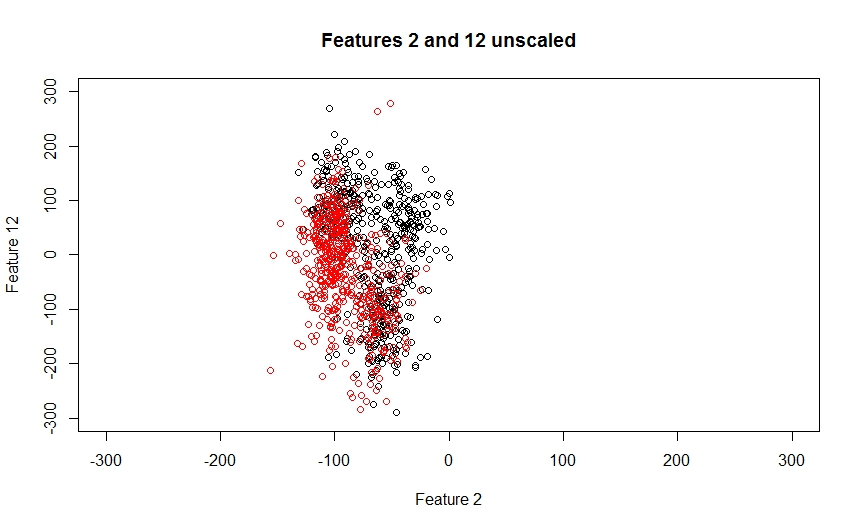
\includegraphics[scale=0.4]{f212.jpeg}
\caption{Features 2 and 12 unscaled; each colour is a class}
\end{figure}

\begin{figure}[H]
\centering
	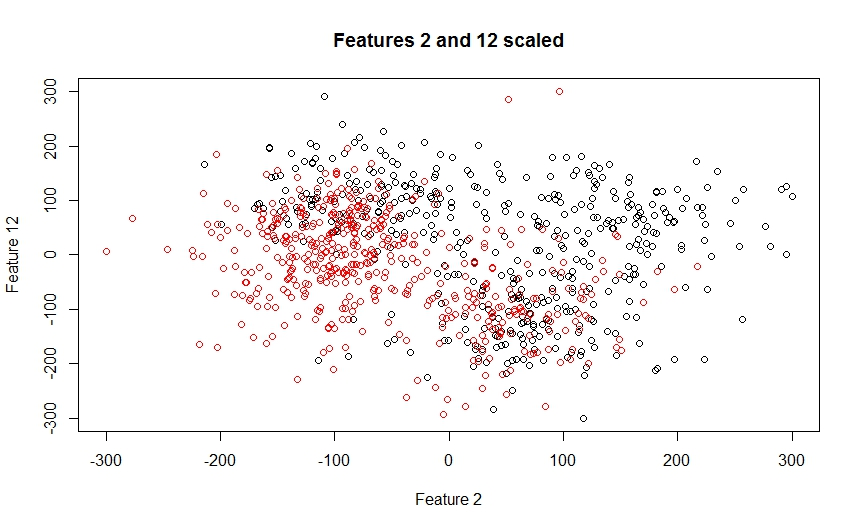
\includegraphics[scale=0.4]{f2122.jpeg}
\caption{Features 2 and 12 scaled; each colour is a class}
\end{figure}

Note that we may also consider a distance-weighted KNN, where the weight of each nearest neighbour is 1 over the distance, but it isn't necessarily more accurate as a classifier. As shown on the following table of hold-out error rates for KNN and distance-weighted KNN used on a section of the data with a few values of $k$, there isn't a clear-cut "better" method in this case.

\begin{tabular}{| l | c | c | c | c | c | c | c | c | c | c |}
\hline
  $k$ & 3 & 5 & 7 & 9 & 11 & 13 & 15 & 17 & 19 \\\hline
  KNN & 0.07 &0.08& 0.07& 0.08& 0.08& 0.05& 0.06& 0.05& 0.07\\\hline
  Distance-weighted KNN & 0.07 &0.06& 0.07& 0.08& 0.07& 0.08& 0.06& 0.07& 0.07 \\\hline
\end{tabular}


So for use with this set of data, we will remain with the simple KNN.

There are two things we must tune: the dimension of the data and the value of $k$ to use. We will first try to reduce the dimension of the data using feature selection. 


\subsubsection{Tuning features: wrapper}
Next we will use the wrapper approach, by assigning a score to each feature by how well the classifier works using that feature. The score is essentially the accuracy rate, i.e. $1 -$ error rate. For the purpose of this method, we will let $k$ be 6.

There are two ways of implementing the wrapper, namely sequential forward and backward selections, each with its advantages and disadvantages. Forward selection's drawback is that once a feature is chosen, it will remain in the chosen set regardless of how well it works with the features chosen later. Backward selection's drawback is that the computation will take a longer time as the number of features evaluated is higher. We will use a combination of both methods to balance out the pros and cons of each. From the 28 features, we will perform forward selection until the score starts decreasing, then narrow it down to 5 and see the optimal number of features that maximises the J-score.

For forward selection, we get the following plot for scores, which peaks at 12. 

\begin{figure}[H]
\centering
	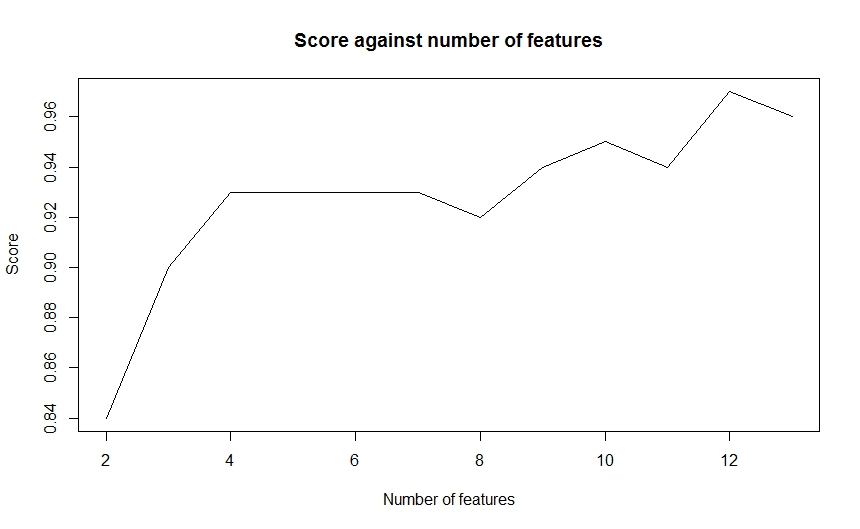
\includegraphics[scale=0.4]{jscore.jpeg}
\caption{Scores; forward selection}
\end{figure}

For backward selection, we get the following plot for scores, which peaks at 9. However it is interesting to note the dip from 11 to 10.

\begin{figure}[H]
\centering
	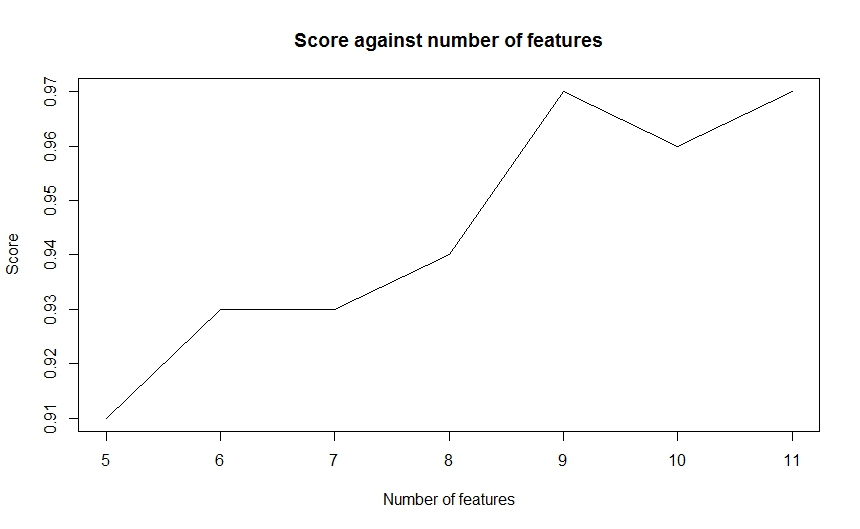
\includegraphics[scale=0.4]{jscore2.jpeg}
\caption{Scores; backward selection}
\end{figure}

The number of features that gives us the highest score is 9, and this algorithm returns us the following list of 10 optimal features to use:

\begin{quote}
\begin{verbatim}
> feature2
                           
 5  4  8  6  3  9  2 14 12   
\end{verbatim}
\end{quote}

Referring back to Figure 1 where we made an informed guess of the features that are likely to be the most and least useful, it seems that the algorithm more or less agrees with our judgment, which, although has no solid weight on its validity, is nonetheless reassuring.

We should note that in theory, the score in sequential forward selection shouldn't decrease then increase again, but in the case of KNN, it is possible that the some features will only prove better if used in conjunction with another as the distance in $n$-dimensions could vary greatly. In light of this, perhaps the wrapper may not be the best method for diminishing the dimension of our data, but we will continue with the selected features as they still improve the overall predictive power of this classifier.


\subsubsection{Tuning parameters: cross-validation}
Next, we will determine the optimal choice of $k$ for this data set based on the 10 selected features, using the out-of-sample error rate produced by leave-one-out cross-validation. Testing values of $k$ from 2 to 50, we get the following plot:

\begin{figure}[H]
\centering
	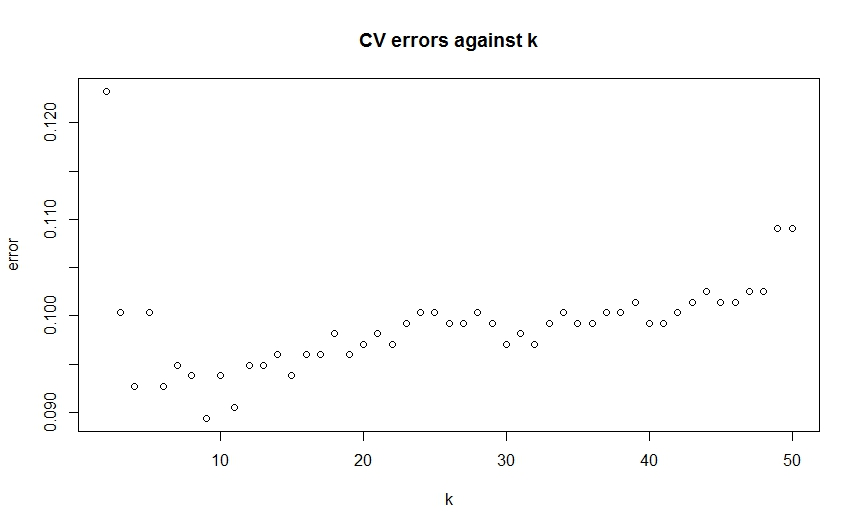
\includegraphics[scale=0.4]{knncv.jpeg}
\caption{Cross-validation errors against $k$}
\end{figure}

We get that the best value of k to use is $k=8$, with an error rate of 0.0894, or 8.94\%.


\subsubsection{Assessment}

\underline{Apparent error}
\\
Using the test set to classify the test set, the apparent error is 0.07633588.

\underline{Hold-out error}
\\
The hold-out error rate is 0.04.

\underline{Leave-one-out cross-validation error}
\\
The leave-one-out cross-validation error is 0.09378408.

\underline{10-fold cross-validation error}
\\
The 10-fold cross-validation error is 0.1010989.


\subsection{Non-linear projection: multi-layer perceptron}

The multi-layer perceptron (MLP) is a feed-forward neural network model. It is a sophisticated classifier in the sense that it projects the data to a lower dimension, in other words attempts to automatically pick out the good features by detecting the correlation between them, so we will try to minimise tampering with our data so that the MLP can take every little detail into account. However, running MLP with all the features returns no results even after a long time as the algorithm fails to find any minima. Hence, we should still try to eliminate a few features, as a lower dimension will greatly decrease the computational load required. We will perform a simple feature selection.

This method's drawback is that it is a "black-box" approach that classifies the data without any understanding of the meaning of the features and hence no indication of class-conditional densities, hence rendering the results difficult to interpret, which in cases such as medicine is more important than the classifications themselves. 

Also, there may be multiple local minima giving different results, and thus we will try several different starting points and either take prediction giving the lowest error rate or take the average scores assigned for predictions.

As we will be using weight decay to prevent over-fitting, we will rescale all the features to the range $[0,1]$ to ensure that the input and the hidden node weights are on the same scale. Note that like KNN, we must remember to re-scale the test set later by the same scales we're using now.

\subsubsection{Tuning features: filter approach}
The filter approach aims to find features with low within-class covariances and high between-class covariance matrices, which are calculated as follows:
\begin{align*}
 \hat{\bSigma}_W &= (\hat{\boldsymbol{s}}_0 + \hat{\boldsymbol{s}}_1)
\\\hat{\bSigma}_B &= \sum_{C=0}^1 \frac{N_C}{N_{TOT}} (\bmu_C - \bmu)(\bmu_C-\bmu)^T
\end{align*}
where

$\hat{\boldsymbol{s}}$ = covariance matrix of class C,
$\\N_c$ = number of points in class C,
$\\\bmu_C$ = sample mean of class C, and
$\\\bmu$ = universal sample mean.

And the score calculated by the trace of the matrix of the inverse of within-class covariance multiplied by between-class covariance. Using the filter, we get the following 13 features:

\begin{quote}
\begin{verbatim}
> feature 
    2    19     6    16     4    17    18     7    12    13     9    24    25 
\end{verbatim}
\end{quote}

On first glance it already doesn't seem right as features 24 and 25 are two of the features we had deemed in Section 1 to be randomly distributed. Testing this on the MLP on several nodes and decay returns us the following hold-out errors:

\begin{quote}
\begin{verbatim}
      decay  nodes  errorrates
 [1,] 1e-03    6       0.11
 [2,] 1e-04    6       0.12
 [3,] 1e-05    6       0.12
 [4,] 1e-03    9       0.13
 [5,] 1e-04    9       0.13
 [6,] 1e-05    9       0.12
 [7,] 1e-03   12       0.10
 [8,] 1e-04   12       0.13
 [9,] 1e-05   12       0.15
\end{verbatim}
\end{quote}

which don't seem great, as testing the same thing on another group of 13 features, 2-14, returns us the following significantly lower hold-out errors:

\begin{quote}
\begin{verbatim}
      decay  nodes  errorrates
 [1,] 1e-03    6       0.10
 [2,] 1e-04    6       0.05
 [3,] 1e-05    6       0.08
 [4,] 1e-03    9       0.07
 [5,] 1e-04    9       0.04
 [6,] 1e-05    9       0.08
 [7,] 1e-03   12       0.10
 [8,] 1e-04   12       0.04
 [9,] 1e-05   12       0.07
\end{verbatim}
\end{quote}

After some consideration, balancing our preference to retain as many useful features as possible and our need to decrease the dimensions, we will select features 2-19 based on our judgment from Figure 1.

\subsubsection{Tuning parameters: trial and error}

There are three things we need to tune: the number of iterations, the number of nodes, and the weight decay. We will let the number of iterations go up to 10000, as most of them converge by then and it takes only about a minute longer than 1000 iterations, so it's a reasonable trade-off between computing time and convergence.

We will use 3 starting points and do two things with it: pick the solution that returns the lowest error rate, and retrieve a solution which is an average of all the predictions, also called \emph{classifier combination}. Using features 2-19, we will test 6, 9 and 12 nodes, and decay of 0.001, 0.0001, and 0.0001. We will retrieve two error rates: the lowest error rate of all three trials, and the error rate of the averaged predictions.
 
The combination that returns us the lowest error rate is 6 nodes and decay of 0.0001, with both the lowest error rate and classifier combination error rate 0.04, but we can see that the errors are very low for others as well.

\begin{quote}
\begin{verbatim}
      decay  nodes errorrates avgerror
 [1,] 1e-03    6       0.07     0.06
 [2,] 1e-04    6       0.04     0.04
 [3,] 1e-05    6       0.07     0.07
 [4,] 1e-03    9       0.05     0.07
 [5,] 1e-04    9       0.05     0.05
 [6,] 1e-05    9       0.07     0.06
 [7,] 1e-03   12       0.07     0.06
 [8,] 1e-04   12       0.07     0.07
 [9,] 1e-05   12       0.06     0.07
\end{verbatim}
\end{quote}

So for this data set we have determined that 6 nodes and decay of 0.0001 is the best combination.

\subsubsection{Assessment}

We will use 5 starting points and use the error rates given by classifier combination.
\\
\\
\underline{Apparent error}
\\
The apparent error rate is 0.006543075.

\underline{Hold-out error}
\\
The hold-out error rate is 0.05.

\underline{Leave-one-out cross-validation error}
\\
The running the leave-one-out cross-validation takes too much machine time so we will omit that.

\underline{10-fold cross-validation error}
\\
The 10-fold cross-validation error rate is 0.07582418.

\subsection{Evaluation of the classifiers}

The following table summarises the error rates for each method in percentage:

\begin{tabular}{| l | c | c | c | c |}
\hline
  Classifier/Type of error & Apparent & Hold-out & CV & 10-fold CV \\\hline
  LDA & 12.76 & 13 & 13.52 & 14.40 \\\hline
  QDA & 6.32 & 9.00 & 8.29 & 8.46 \\\hline
  KNN & 7.63 & 4 & 9.38 & 10.11 \\\hline
  MLP & 0.65 & 5 & - & 7.58 \\
  \hline
\end{tabular}

We know that the apparent error gives a biased performance estimate, as it assesses the same data that it had used to form the classifier, but we will keep it there simply as a reference. The hold-out error gives an unbiased performance estimate, but makes inefficient use of the data, as it doesn't take make use of as much data as it could have. In theory, the hold-out error should be less than the cross-validation error, but as we can see here this is not necessarily the case. For KNN and MLP, we could perhaps attribute it to the fact that we had used hold-out errors as a basis score for feature and parameter selection. The leave-one-out cross validation error doesn't have the same problem, but is computationally demanding, and for this reason, omitted for MLP. 

It seems that the 10-fold cross-validation error is the most suitable error upon which to judge the classifiers, as it is less biased than other errors and is possible to computed within a reasonable time. Based on this error, we say that QDA and MLP are the best classifiers among all in this scenario.

\section{Using the test set}
Now we compare our best two classification methods on our test set using McNemar's test at the 1\% significance level, which means that we reject the null hypothesis that the tests have the same error if $|z| > 2.58$. 

We get that the test statistic is 0.7559289, so we have little reason to reject the null hypothesis. Hence we conclude with 99\% significance level that the two classifiers are equally good.

\section{Recommendation}

Each classifier has its strengths and weaknesses, but taking all into consideration, we would recommend QDA. QDA contains all the advantages of LDA in that it is a machine learner, simple to code, quick to run, gives us more information than just classifications, plus the reduced constraints and assumptions mean that it could fit the data better. The main drawback of QDA, it requiring large amounts of data to work well, doesn't apply here as we have a large data set.

Although MLP is much more sophisticated, performs automatic feature extraction, and has lower error rates than QDA, its drawbacks are also numerous. It takes a significantly longer computing time than the rest in terms of training time, so much that when applied on the entire data set with all the features, it fails to find local minimas after many tries and results in the code looping endlessly. MLP also requires careful handling in terms of re-scaling the data and selecting parameters, neither of which are difficult but mistakes can easily be made resulting in parameters not being optimised. Moreover, MLP focuses only on classification, and it does not give us any other information regarding the data, for example the prior distributions. 

In considering the best classifier to use, prediction accuracy is the important factor, but other factors also have their own weights. Based on the McNemar test for 1\% significance level, QDA and MLP are on par with each other performance-wise. Hence, we would select QDA to be the most appropriate out of the above classifiers as it is a good trade-off between classification accuracy, complexity, computing time, and interpretability.


\newpage
\section{Appendix A}

Below is the code used in the report.

Organising data
\begin{quote}
\begin{verbatim}
#' Cissy Chan
#' Statistical Pattern Recognition
#' M3S7
#' January 2014 

# all the packages used in this script, uncomment if they aren't already installed
#install.packages(c("mvnmle", "matrixcalc", "nnet", "MASS", "stats", "class"))

library(mvnmle)
library(matrixcalc)
library(nnet)
library(MASS)
library(stats)
library(class)

# read data
data6 <- utils::read.table(
  "http://www2.imperial.ac.uk/~eakc07/S7/data6.dat",
  header=FALSE,
  sep=" ",
  na.strings="NA",
  dec=".",
  strip.white=TRUE
)
#View(data6)

# split into training and test samples
# we will not touch this test sample until the very end
set.seed(1)
v1 <- sample(1:1102, 100, FALSE)
te <- data6[v1, ]
tr <- data6[-v1, ]

# plot all the feature vectors to get a rough idea of what we're dealing with
par(mfrow=c(4, 4),mar=c(1, 2, 2, 1))
for (i in 2:17) {
  plot(tr[, i], xaxt="n", frame.plot=TRUE, main=as.character(i))
}

par(mfrow=c(4,4), mar=c(1, 2, 2, 1))
for (i in 18:29) {
  plot(tr[, i], xaxt="n", frame.plot=TRUE, main=as.character(i))
}

# pick out all the NA values
isna <- is.na(tr)
# see which features have the NA values
colSums(isna)
# see how many NA values each observation has
max(rowSums(isna))
# so each has max. of 1 NA. How many obs contain NA?
sum(isna)
# 85 out of 1002. There are ways to deal with this, like substituting 
# the data with the mean, or conditional mean
# However I think we can afford to get rid of that
trfull <- tr[complete.cases(tr), ]
#oh and check that it's not mostly biased towards one class
dim(trfull[trfull[, 1]==0, ])

dev.off()
\end{verbatim}
\end{quote}

LDA
\begin{quote}
\begin{verbatim}
#---------------------------------------------------------------------------
# Linear discriminant analysis
#---------------------------------------------------------------------------

# split data into training (tr1) and test (tr2)
set.seed(1)
v <- sample(1:nrow(trfull), 100, FALSE)
tr1 <- data.frame(trfull[-v, ])
tr2 <- data.frame(trfull[v, ])

# set up function to assign scores for each feature
filter2 <- function(a) {
  lda1 <- lda(as.matrix(trfull[,a]), trfull[, 1], CV=TRUE)$class
  e <- sum(lda1 == trfull[, 1]) / nrow(trfull)
  
  return(e)
}

range <- matrix(2:29, ncol=1)

# run features through filter and plot scores
a <- apply(range, 1, filter2)
plot(range, a, main="Score for each feature", xlab="Features", ylab="Score")

b <- cbind(a, 2:29)
o <- order(b[, 1], decreasing=T)

# set up function to test LDA against increasing number of features
a <- function(d) {
  c <- b[o, ][1:d, 2]  
  lda1 <- lda(as.matrix(trfull[,c]), trfull[, 1], CV=TRUE)$class
  e <- sum(lda1 != trfull[, 1]) / nrow(trfull)
  
  return(e)
}

# run features through function and plot scores
f1 <- apply(as.matrix(2:28), 1, a)
plot(
  x=2:28,
  y=f1,
  main="CV error against number of features",
  xlab="Number of features",
  ylab="CV error"
)

# get the number of features that gives minimum score
which.min(f1)

# the optimal features
c <- b[o, ][1:(which.min(f1)+1), 2]
c

# apparent error
lda1 <- lda(trfull[, c], trfull[, 1])
lda2 <- predict(lda1, trfull[, c])$class
sum(lda2 != trfull[, 1]) / nrow(trfull)

# hold-out error
lda1 <- lda(as.matrix(tr1[, c]), tr1[, 1])
lda2 <- predict(lda1, as.matrix(tr2[, c]))$class
sum(lda2 != tr2[, 1]) / nrow(tr2)

# CV error
lda1 <- lda(as.matrix(trfull[, c]), trfull[, 1], CV=TRUE)$class
sum(lda1 != trfull[, 1]) / nrow(trfull)

# CV all features
lda1 <- lda(as.matrix(trfull[, 2:29]), trfull[, 1], CV=TRUE)$class
sum(lda1 != trfull[, 1])/nrow(trfull)

# 10-fold cv
a <- matrix(0, ncol=10, nrow=91)
b <- 1
count <- 1
while(count < 11) {
  set.seed(1)
  a[, count] <- sample((1:917)[-b],91,FALSE)
  b <- matrix(a[, 1:count], ncol=1)
  count <- count + 1
}

tenfoldlda <- function(d) {
  k <- matrix(a[, -d], ncol=1)
  lda1 <- lda(as.matrix(trfull[k, c]),trfull[k, 1])
  lda2 <- predict(lda1, as.matrix(trfull[a[, d], c]))$class
  error<- sum(lda2 != trfull[a[, d], 1])/nrow(trfull[a[, d], ])
  list(error = error)
}

e <- apply(as.matrix(1:10), 1, tenfoldlda)
errorrates <- numeric(10)
for (i in 1:10) {errorrates[i] <- e[[i]]$error}
sum(errorrates)/10
\end{verbatim}
\end{quote}

QDA
\begin{quote}
\begin{verbatim}
#---------------------------------------------------------------------------
# Quadratic discriminant analysis
#---------------------------------------------------------------------------

filter2 <- function(a) {
  qda1 <- qda(as.matrix(trfull[, a]), trfull[, 1], CV=TRUE)$class
  e <- sum(qda1 == trfull[, 1])/nrow(trfull)
  
  return(e)
}

range <- matrix(2:29, ncol=1)

a <- apply(range, 1, filter2)
plot(range, a, main="Score for each feature", xlab="Features", ylab="Score")

b <- cbind(a, 2:29)
o <- order(b[, 1], decreasing=T)

a <- function(d) {
  c <- b[o, ][1:d, 2]  
  qda1 <- qda(as.matrix(trfull[, c]), trfull[, 1], CV=TRUE)$class
  e <- sum(qda1 != trfull[, 1])/nrow(trfull)
  return(e)
}
f1 <- apply(as.matrix(2:28), 1, a)
plot(
  x=2:28,
  y=f1,
  main="CV error against number of features",
  xlab="Number of features",
  ylab="CV error"
)
which.min(f1)

# the optimal features
c <- b[o, ][1:(which.min(f1)+1), 2]
c

# apparent error
qda1 <- qda(trfull[, c], trfull[, 1])
qda2 <- predict(qda1, trfull[, c])$class
sum(qda2 != trfull[, 1])/nrow(trfull) 

# hold-out error
qda1 <- qda(as.matrix(tr1[, c]),tr1[, 1])
qda2 <- predict(qda1, as.matrix(tr2[, c]))$class
sum(qda2 != tr2[, 1])/nrow(tr2) 

# CV error
qda1 <- qda(as.matrix(trfull[, c]),trfull[, 1], CV=TRUE)$class
sum(qda1 != trfull[, 1])/nrow(trfull)

# CV all features
qda1 <- qda(as.matrix(trfull[, 2:29]), trfull[, 1], CV=TRUE)$class
sum(qda1 != trfull[, 1])/nrow(trfull)

# 10-fold cv
a <- matrix(0, ncol=10, nrow=91)
b <- 1
count <- 1
while(count < 11) {
  set.seed(1)
  a[, count] <- sample((1:917)[-b], 91, FALSE)
  b <- matrix(a[, 1:count], ncol=1)
  count <- count + 1
}

tenfoldqda <- function(d) {
  k <- matrix(a[, -d], ncol=1)
  qda1 <- qda(as.matrix(trfull[k, c]), trfull[k, 1])
  qda2 <- predict(qda1, as.matrix(trfull[a[, d], c]))$class
  error<- sum(qda2 != trfull[a[, d], 1])/nrow(trfull[a[, d], ])
  list(error = error)
}

e <- apply(as.matrix(1:10), 1, tenfoldqda)
errorrates <- numeric(10)
for (i in 1:10) {errorrates[i] <- e[[i]]$error}
sum(errorrates)/10

qdafeatures <- c
\end{verbatim}
\end{quote}

KNN
\begin{quote}
\begin{verbatim}
#---------------------------------------------------------------------------
# K nearest neighbours
#---------------------------------------------------------------------------

plot(
  x=tr[tr[, 1]==0, 2],
  y=tr[tr[, 1]==0, 12],
  xlab="Feature 2",
  ylab="Feature 12",
  main="Features 2 and 12 unscaled",
  xlim=c(-300, 300),
  ylim=c(-300, 300)
)
points(tr[tr[, 1]==1, 2], tr[tr[, 1]==1, 12], col=2)

# rescaling the data
trknn <- trfull
rescale <- function(x) (x - min(x))/(max(x) - min(x)) * 600 - 300
trknn[, -1] <- apply(trfull[, -1], 2, rescale)

plot(
  x=trknn[trknn[, 1]==0, 2],
  y=trknn[trknn[, 1]==0, 12],
  xlab="Feature 2",
  ylab="Feature 12",
  main="Features 2 and 12 scaled",
  xlim=c(-300, 300),
  ylim=c(-300, 300)
)
points(trknn[trknn[, 1]==1, 2], trknn[trknn[, 1]==1, 12], col=2)

set.seed(1)
v <- sample(1:nrow(trknn), 100, FALSE)
trk1 <- data.frame(trknn[-v, ])
trk2 <- data.frame(trknn[v, ])

# knn for wrapper
knnwrap <- function(r) {
  set.seed(1)
  x <- knn(as.matrix(trk1[, r]), as.matrix(trk2[, r]), trk1[, 1], 6)
  J <- sum(x == trk2[, 1])/nrow(trk2)
  return(J)
}

# WRAPPER
range <- matrix(2:29, ncol=1)

top <- 13

a <- apply(range, 1, knnwrap)
feature <- range[which.max(a)]
jscore <- numeric(top)
range <- range[-which.max(a)] #remove the row with lowest J score
newrange <- cbind(rep(feature, length(range)), range)


while(length(feature) < top) {
  a <- apply(newrange, 1, knnwrap)
  feature <- newrange[which.max(a), ]
  jscore[length(feature)] <- max(a)
  range <- range[-which.max(a)]
  newrange <- cbind(t(matrix(rep(feature, length(range)),
                             nrow=length(feature))), range)
}

plot(
  x=2:top,
  y=jscore[-1],
  type="l",
  main="Score against number of features",
  xlab="Number of features",
  ylab="Score"
)

feature <- feature[1:top-1]
feature1 <- feature

jscore2<- numeric(top-2)

while(length(feature) > 9) {
  a <- t(matrix(feature, nrow=length(feature), ncol=length(feature)))
  diag(a) <- NA
  a <- t(a)
  range <- t(matrix(a[!is.na(a)], nrow=length(feature)-1, ncol=length(feature)))
  b <- apply(range, 1, knnwrap)
  feature <- feature[-which.max(b)]
  jscore2[length(feature)] <- max(b)
}

feature2 <- feature
feature2

while(length(feature) > 5) {
  a <- t(matrix(feature, nrow=length(feature), ncol=length(feature)))
  diag(a) <- NA
  a <- t(a)
  range <- t(matrix(a[!is.na(a)], nrow=length(feature)-1, ncol=length(feature)))
  b <- apply(range, 1, knnwrap)
  feature <- feature[-which.max(b)]
  jscore2[length(feature)] <- max(b)
}

feature1

plot(
  x=5:(top-2),
  y=jscore2[-(1:4)],
  type="l",
  main="Score against number of features",
  xlab="Number of features",
  ylab="Score"
)


knncv <- function(k) {
  set.seed(1)
  w <- knn.cv(trknn[, feature2], trknn[, 1], k)
  error <- sum(w != trknn[, 1])/nrow(trknn)
  return(error)
}

k <- matrix(2:50)
error <- apply(k, 1, knncv)
plot(k, error, main="CV errors against k")
which.min(error)
min(error)

#apparent error
set.seed(1)
w <- knn(trknn[, feature2], trknn[, feature2], trknn[, 1], 8)
sum(w!=trknn[, 1])/nrow(trknn)

#hold-out error
set.seed(1)
w <- knn(trk1[, feature2], trk2[, feature2], trk1[, 1], 8)
sum(w!=trk2[, 1])/nrow(trk2)

#cv error
set.seed(1)
w <- knn.cv(trknn[, feature2], trknn[, 1], 8)
sum(w!=trknn[, 1])/nrow(trknn)

#10-fold cv
a <- matrix(0, ncol=10, nrow=91)
b <- 1
count <- 1
while(count < 11) {
  set.seed(1)
  a[,count] <- sample((1:917)[-b], 91, FALSE)
  b <- matrix(a[, 1:count],ncol=1)
  count <- count + 1
}

tenfoldknn <- function(d) {
  j <- matrix(a[,-d], ncol=1)
  set.seed(1)
  w <- knn(trknn[j, feature2], trknn[a[, d], feature2], trknn[j, 1], 8)
  error <- sum(w!=trknn[a[, d], 1])/nrow(trknn[a[, d] , ])
  list(error = error)
}

e <- apply(as.matrix(1:10), 1, tenfoldknn)
errorrates <- numeric(10)
for (i in 1:10) {errorrates[i] <- e[[i]]$error}
sum(errorrates)/10
\end{verbatim}
\end{quote}

Distance-weighted KNN
\begin{quote}
\begin{verbatim}
train <- trk1[, 2:19]
test <- trk2[, 2:19]
class <- trk1[, 1]
classte <- trk2[, 1]

p <- ncol(train)
ntr <- nrow(train)
nte <- nrow(test)
ngroups <- 2

knn.dist <- function(k) {
  
  k <- k + 1
  
  class1 <- array(0, nte)
  
  for (i in 1:nte) {
    a <- array(0,dim=c(2, p, ntr))
    a[1, , ] <- rep(test[i, ], ntr)
    a <- array(a,dim=c(2, p, ntr))
    a[2, , ] <- t(train)
    
    d1 <- apply(a, 3, function(x) abs(dist(x, method="euclidean")))
    d <- cbind(d1, class)
    o <- order(d[, 1], decreasing=F)
    kmin1 <- d[o, ][(1:k), ]
    
    if (kmin1[k, 1]>0) {
      kmin <- cbind(kmin1[, 1]/kmin1[k, 1],kmin1[, 2])
    }
    
    w <- kmin
    w[, 1] <- apply(t(kmin[, 1]), 1,function(x) (1/x))
    w <- kmin1
    
    b <- array(0, dim=c(ngroups, 1))
    
    b[1] <- sum(w[, 1]*(w[, 2]==0))
    b[2] <- sum(w[, 1]*(w[, 2]==1))
    
    class1[i] <- c(0, 1)[which.max(b)]
  }
  error <- sum(class1 != classte)/nte
  return(error)
  
}

knnall <- function(k) {
  set.seed(1)
  a <- knn(train, test, class, k)
  return(sum(a != classte)/nte)
}
#distance-weighted knn
a <- apply(as.matrix(seq(3, 19, 2)), 1, knn.dist)
#knn
b <-apply(as.matrix(seq(3, 19, 2)), 1, knnall)
\end{verbatim}
\end{quote}

MLP
\begin{quote}
\begin{verbatim}
#---------------------------------------------------------------------------
# Multi-layer perceptron
#---------------------------------------------------------------------------

#filter
filter1 <- function(a) {
  s0 <- var(trfull[trfull[, 1]==0, a])
  s1 <- var(trfull[trfull[, 1]==1, a])
  SW <- s0 + s1
  m0 <- mean(trfull[trfull[, 1]==0, a])
  m1 <- mean(trfull[trfull[, 1]==1, a])
  m <- mean(trfull[,a])
  SB <- nrow(trfull[trfull[, 1]==0, ]) / nrow(trfull) * (m0-m) %*% t(m0-m) + 
    nrow(trfull[trfull[, 1]==1, ])/nrow(trfull) * (m1-m) %*% t(m1-m)
  
  J <- Matrix::solve(SW) %*% SB
  
  return(J)  
}

filter <- function(a) {
  s0 <- mlest(trfull[trfull[, 1]==0, a])$sigmahat
  s1 <- mlest(trfull[trfull[, 1]==1, a])$sigmahat
  SW <- s0 + s1
  m0 <- mlest(trfull[trfull[, 1]==0, a])$muhat
  m1 <- mlest(trfull[trfull[, 1]==1, a])$muhat
  m <- mlest(trfull[,a])$muhat
  SB <- nrow(trfull[trfull[, 1]==0, ])/nrow(trfull) * (m0-m) %*% t(m0-m) + 
    nrow(trfull[trfull[, 1]==1, ])/nrow(trfull) * (m1-m) %*% t(m1-m)
  
  J <- matrix.trace(Matrix::solve(SW) %*% SB)
  
  return(J)
}

range <- matrix(2:28)
a <- apply(range, 1, filter1)
feature <- range[which.max(a)]
jscore <- numeric(28)
range <- range[-which.max(a)] #remove the row with lowest J score
newrange <- cbind(rep(feature, length(range)), range)

while(length(feature) < 13) {
  a <- apply(newrange, 1, filter)
  feature <- newrange[which.max(a), ]
  jscore[length(feature)] <- max(a)
  range <- range[-which.max(a)]
  newrange <- cbind(t(matrix(rep(feature, length(range)), nrow=length(feature))), range)
}

feature


"which.is.min" <-
  function(x)
  {
    y <- seq(along = x)[x == min(x)]
    if(length(y) > 1)
      sample(y, 1)
    else y
  }

trmlp <- trfull
rescale <- function(x) (x - min(x))/(max(x) - min(x))
trmlp[, -1] <- apply(trfull[, -1], 2, rescale)

set.seed(1)
v <- sample(1:nrow(trmlp), 100, FALSE)
trm1 <- data.frame(trmlp[-v, ])
trm2 <- data.frame(trmlp[v, ])

H <- c(6, 9, 12)
wd <- c(0.001, 0.0001, 0.00001)
gr <- as.matrix(expand.grid(wd,H))

# MLP with one hidden layer
"nnet.f" <-
  function(x, ntry)
  {
    set.seed(1)
    H <- x[2]
    decay <- x[1]
    preds <- matrix(0,ncol=ntry,nrow=nrow(trm2))
    score <- numeric(ntry)
    count <- 0
    while(count < ntry) {
      mlp <- nnet(trm1[, 2:19], trm1[, 1], size=H, decay=decay, maxit=10000)
      evs <- eigen(nnetHess(mlp, trm1[, 2:19],trm1[, 1]), TRUE)$values
      #ensures that this is a minima; evalues of Hessian all > 0
      if(min(evs) > 0) {
        count <- count + 1
        preds[, count] <- as.numeric(predict(mlp, trm2[, 2:19]))
        score[count] <- sum((preds[, count] > 0.5) != trm2[, 1])/nrow(trm2)
      }
    }
    avgscore <- sum((rowSums(preds) > 0.5*ntry) != trm2[, 1])/nrow(trm2)
    indx <- which.is.min(score)
    list(score = score[indx], avgscore = avgscore)
  }

a <- apply(gr, 1, nnet.f,ntry=3) #3 different starting points
errorrates <- avgerror <- numeric(9)
for (i in 1:9) {errorrates[i] <- a[[i]]$score
               avgerror[i] <- a[[i]]$avgscore}
min(errorrates)
gr[which.min(errorrates), ]
grid <- cbind(gr, errorrates, avgerror)

# holdout error
ntry <- 5
preds <- matrix(0, ncol=ntry, nrow=nrow(trm2))
score <- numeric(ntry)
count <- 0
set.seed(1)
while(count < ntry) {
  mlp <- nnet(trm1[, (2:19)], trm1[, 1], size=6, decay=0.0001, maxit=10000)
  evs <- eigen(nnetHess(mlp, trm1[, (2:19)], trm1[, 1]), TRUE)$values
  # ensures that this is a minima; evalues of Hessian all > 0
  if(min(evs) > 0) {
    count <- count + 1
    preds[, count] <- as.numeric(predict(mlp, trm2[, (2:19)]))
  }
}
ho <- sum((rowSums(preds) > 0.5*ntry) != trm2[, 1])/nrow(trm2)
ho

# 10-fold cv
a <- matrix(0, ncol=10, nrow=91)
b <- 1
count <- 1
while(count < 11) {
  set.seed(1)
  a[,count] <- sample((1:917)[-b], 91, FALSE)
  b <- matrix(a[, 1:count], ncol=1)
  count <- count + 1
}

tenfold <- function(c) {
  set.seed(1)
  preds <- matrix(0, ncol=ntry, nrow=nrow(trmlp))
  score <- numeric(1)
  count <- 0
  while(count < ntry) {
    k <- matrix(a[, -c], ncol=1)
    mlp <- nnet(trmlp[k, 2:19], trmlp[k, 1], size=6, decay=0.0001, maxit=10000)
    evs <- eigen(nnetHess(mlp, trmlp[k, 2:19], trmlp[k, 1]),TRUE)$values
    #ensures that this is a minima; evalues of Hessian all > 0
    if(min(evs) > 0) {
      count <- count + 1
      preds <- as.numeric(predict(mlp, trmlp[a[, c], 2:19]))
      score[count] <- sum((preds > 0.5) != trmlp[a[, c], 1])/nrow(trmlp[a[, c], ])
    }
  }
  indx <- which.is.min(score)
  list(score = score[indx])
}

a <- apply(as.matrix(1:10), 1, tenfold)
errorrates <- numeric(10)
for (i in 1:10) { errorrates[i] <- a[[i]]$score }
tencv <- sum(errorrates)/10
tencv

# mcnemar
te <- te[complete.cases(te), ]

# qda
qda1 <- qda(trfull[, qdafeatures], trfull[, 1])
qdapredict <- predict(qda1, te[, qdafeatures])$class

# rescaling data for mlp the same way we did it for training set
tem <- te
rescale <- function(x, min, max) ((x - min)/(max - min))
for (i in 2:29) {
  tem[, i] <- rescale(te[, i], min(trfull[, i]), max(trfull[, i]))
}

# mlp
ntry <- 5
preds <- matrix(0, ncol=ntry, nrow=nrow(tem))
score <- numeric(ntry)
count <- 0
set.seed(1)
while(count < ntry) {
  mlp <- nnet(trmlp[, (2:19)], trmlp[, 1], size=6,decay=0.0001, maxit=10000)
  evs <- eigen(nnetHess(mlp, trmlp[, (2:19)], trmlp[, 1]), TRUE)$values
  # ensures that this is a minima; evalues of Hessian all > 0
  if(min(evs) > 0) {
    count <- count + 1
    preds[, count] <- predict(mlp, tem[, (2:19)])
  }
}

mlppredict <- as.numeric((rowSums(preds) > 0.5*5))

mcnemar <- function(s) {
  p <- s[1]
  q <- s[2]
  r <- s[3]
  if (p != q & q == r) {
    return(0)
  }
  if (p != q & p == r) {
    return(1)
  }
  if (p != r & p == q) {
    return(2)
  }
  if (p == q & p == r) {
    return(3)
  }
}

qdapredict <- as.numeric(qdapredict)
if(min(qdapredict) == 1) {
  qdapredict <- qdapredict -1
}
s <- cbind(te[, 1], qdapredict, mlppredict)
h <- apply(s, 1, mcnemar)
n00 <- sum(h==0)
n01 <- sum(h==1)
n10 <- sum(h==2)
n11 <- sum(h==3)

z <- (abs(n01 - n10) - 1)/(sqrt(n10 + n01))
z
\end{verbatim}
\end{quote}

\end{document}